% SLIDE
\begin{frame}
	\frametitle{Context}
	\begin{itemize}
		\item Competitive FPS depend on technical fairness: same rules, same information, for all players
		\item High stakes: esports prize pools (\$75 million at the 2026 EWC), professional careers, ranked progression
		\item Cheating (aimbots, wallhacks) directly threatens this integrity
	\end{itemize}
\end{frame}

% SLIDE
\begin{frame}
	\frametitle{The industry's answer, and its cost}
	\begin{itemize}
		\item Publishers responded with kernel-level (Ring 0) anti-cheat: full system visibility to catch cheats
		\item But: this grants a third-party driver unrestricted access to the entire machine, not just the game
		\item Raises real cybersecurity and privacy concerns
	\end{itemize}
	% \begin{center}
	% 	\hspace{-10mm}
	%   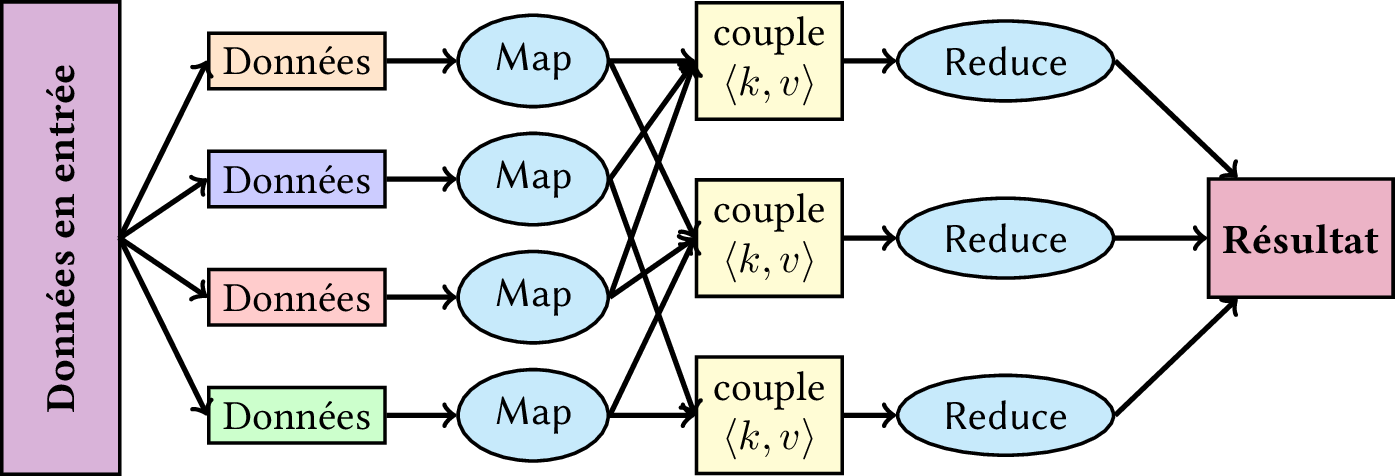
\includegraphics[height=2.7cm]{../images/Mapreduce.png}
	% 	\vspace*{-3mm}
	% \end{center}
\end{frame}

% SLIDE
\begin{frame}
	\frametitle{Problem}
	\begin{center}
		How can we detect cheating effectively without compromising system security through kernel-level access?
	\end{center}
\end{frame}
